\section{LEGO NXT Operating Systems}
The NXT is shipped with LEGO's own operating system, which LEGO has released as open source. There are however several other open source operating systems that provide other features. 

\subsection{Operating System Alternatives} % (fold)
\label{sub:opertating_system_alternatives}
Among the commonly used operating systems are leJOS and nxtOSEK.

nxtOSEK~\cite{osek_os} is a open source real-time operating system based on the OSEK specification~\cite{osek_spec}, it requires a custom firmware for the NXT brick.

nxtOSEK comes with features that enable ANSI C/C++ programming using a GCC compiler. It also includes a C/C++ API for NXT sensors, motor and other devices, which makes it possible to interact with the LEGO Mindstorms platform. nxtOSEK comes with TOPPERS/JSP (Just Standard Profile) which is a real time kernel written in C that provides real time multitasking features. nxtOSEK provides a wide variety of features such as task management, synchronization, interrupt management, alarms, intra processor message handling and error treatment. Some of the features that might be useful in the context of this project will be described briefly in the following section. 

LeJOS is a small Java Virtual Machine that can be ported to the LEGO NXT brick\cite{lejos}. LeJOS provides object oriented programming in the form of the Java programming environment. It also provides real-time functionality such as preemptive tasks, recursion, synchronization, exceptions, Java types (including float, long and String), single and multidimensional arrays etc. 

The group decided to focus on the OSEK operating system given that it has received an introductory lecture on OSEK and there is substantial support to be obtained on campus for this OS.
% subsection opertating_system_alternatives (end)

\subsection{Task management in OSEK} % (fold)
\label{sub:task_management_in_osek}
Tasks are a convenient way of dividing complex control software according to their real time requirements. Tasks provide the framework for the execution of functions. 
The nxtOSEK operating system supports two types of tasks, basic and extended tasks and nxtOSEK has its own scheduler. \autoref{taskstate} shows an overview of the different states that the two types of tasks can be in.

\begin{figure}[hptb]
  \centering
    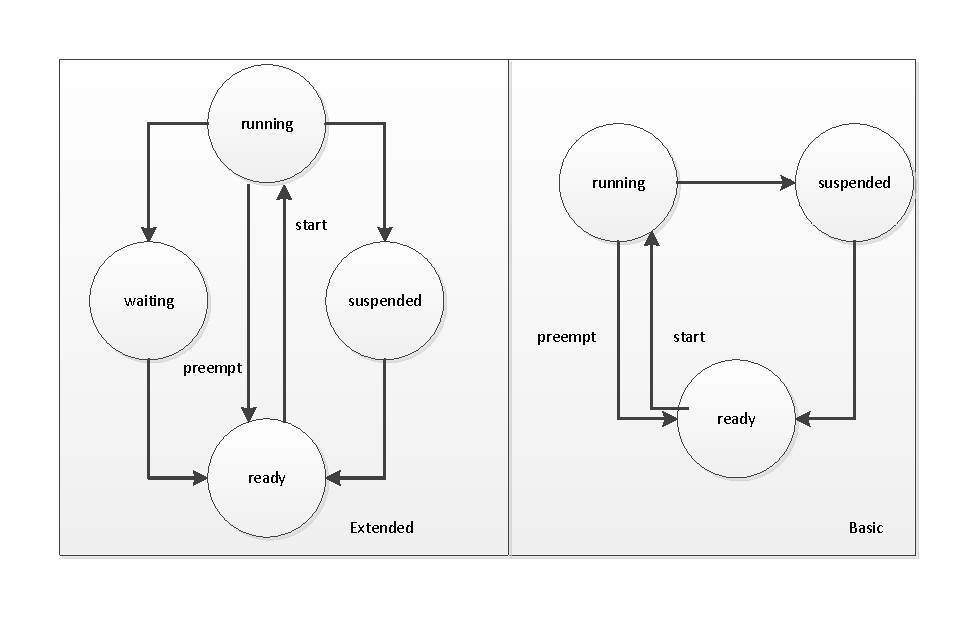
\includegraphics[width=1.0\textwidth]{img/taskstate.pdf}
  \caption{Basic and extended tasks and their states.}
  \label{taskstate}
\end{figure}

\textbf{Basic tasks} only release the processor if they terminate, if the OS switches to a task with a higher priority or if the task gets an interrupt.
\textbf{Extended tasks} are distinguished from basic tasks by the fact that they can use the call \emph{WaitEvent}, which sets the task in a \emph{waiting} state and releases the processor without terminating the task and allows lower priority tasks to access the processor.

\subsection{Scheduling in nxtOSEK} % (fold)
\label{sub:scheduling_in_nxtosek}
 Scheduling is vital when the number of tasks in a program start to increase. There are several types of scheduling, but the main question is whether there is preemption or not. Preemption is when a low priority task gets paused to allow a higher priority task to execute instead. When the high priority task is done, the lower priority task can resume its execution. This behavior has i's pros and cons, on one hand it is beneficial to have the most important tasks executing as quickly as possible, but on the other hand this could lead to starvation of low priority tasks as there may be many tasks with higher priority, hence the low priority task would never execute. 

nxtOSEK supports both full preemptive and non preemptive scheduling. It also supports hybrids of the two in "groups of tasks" and mixed preemptive scheduling.

\textbf{Groups of tasks} combines aspects of preemptive and non preemptive behavior. Task are gathered in groups and for tasks that have a priority lower or equal to the group's highest priority the tasks within the group have non preemptive behaviour. To tasks with higher priority than the group's highest priority, the tasks within the group have preemptive behaviour. In other words if the task has higher priority than the group, then the tasks within the group are preemptive otherwise they are non preemptive.

\textbf{Mixed preemptive scheduling} is exactly what the name suggests. The system contains both preemptive and non preemptive tasks. The active scheduling scheme depends on the task that is executing. If the running task is preemptive, preemptive scheduling is performed. If the running task is non preemptive, then non preemptive scheduling is performed. 

General scheduling selection is done by specifying task priorities and assigning preemption as attributes. The task type (basic or extended) is independent of the scheduling policy. 
% subsection scheduling_in_nxtosek (end)
% subsection task_management_in_osek (end)
